%%%%%%%%%%%%%%%%%%%%%%%%%%%%%%%%%%%%%%%%%%%%%%%%%%%%%%%%%%%%%%%
%
% Welcome to Overleaf --- just edit your LaTeX on the left,
% and we'll compile it for you on the right. If you give
% someone the link to this page, they can edit at the same
% time. See the help menu above for more info. Enjoy!
%
% Note: you can export the pdf to see the result at full
% resolution.
%
%%%%%%%%%%%%%%%%%%%%%%%%%%%%%%%%%%%%%%%%%%%%%%%%%%%%%%%%%%%%%%%
% Nested Grids in SWAN and WAM coupling
% Author: Marco Miani
% Nested grid and nesting play a crucial role in SWAN model. Lack of resolution is a 
% main problem. SWAN overcomes it, by interpolating a denser grid. 
\documentclass[12pt]{article}
\usepackage{tikz}


\usetikzlibrary{positioning}
\usetikzlibrary{trees}
\usetikzlibrary{decorations.pathmorphing}
\usetikzlibrary{decorations.markings}
\usetikzlibrary{decorations.pathreplacing,decorations.pathmorphing}




\begin{document}
%\pagestyle{empty}
\begin{figure}[t!]
    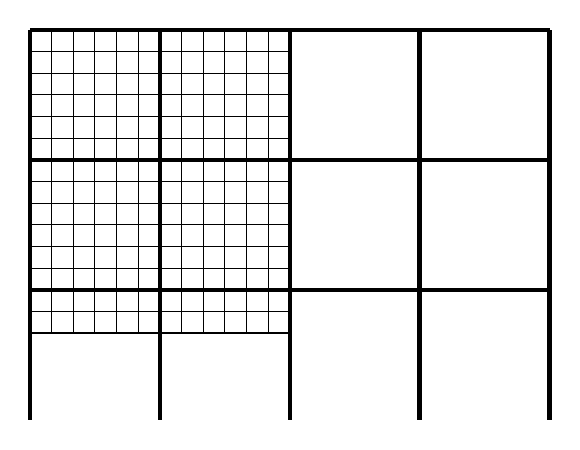
\begin{tikzpicture}[scale=.55,interface/.style={
            postaction={draw,decorate,decoration={border,angle=45,
                        amplitude=0.5cm,segment length=3mm}}}]
    
    
        \begin{scope}%[xshift=-100mm,
        %yshift=90,every node/.append style={
        %yslant=0.0,xslant=0},yslant=0.,xslant=0
         %            ]
        %\fill[white,fill opacity=.9] (0,0) rectangle (7,9);
    %Coarse grid is obtained by drawins subgridS and puzzling them together. 
    %\draw[step=20mm,black,thick] (2,0) grid (6,6); 
    %\draw[step=20mm,black,thick] (6,5) grid (9,6); 
    
    %\draw[step=20mm,black,thick] (0,5) grid (2,-3.0);%XXXXXX
    %\draw[step=20mm,black,thick] (0,5.0) grid (2,6); 
    
    \draw[step=30mm,black,ultra thick] (0,-3) grid (12,6);

    %nested grid
    \draw[step=5mm, black] (0,-1) grid (6,6);
    
    %filling
    %\fill[red,ultra thick] (6.1,6.1) rectangle (7.9,7.9);%cell element


    \end{scope}
    
    \end{tikzpicture}

\end{figure}
\end{document}